\chapter{Related Work}
\label{ch:related}

\section{Literature Studies}
Currently, there exists no specific suggestions on how to optimally use the SMACK-stack in the aspect of resource distribution between the individual technologies.
Further this thesis focuses on the scalability of the whole stack and aims to find bottlenecks when dealing with various input data patterns.
There is research for each of the technologies but not in their combination, and especially there are no recommendations based on empirical experiments for how to setup the stack optimally with a given budget and specific requirements.

\subsection{Cloud Computing \& Big Data}
There is a lot of research in the field of cloud computing and big data.
In their paper "Fast Data in the Era of Big Data" Mishne et al. show the background of Twitters new spelling correction and query suggestion, which has the demand to include recent events within minutes \cite{mishne2013fast}.
The approach shows that the commonly used Hadoop-based approach did not work out well, as the provided latency was simply to high.
In the final result they build their own in-memory processing engine, to be able to handle data faster.
This is similar to Apache Spark, as it also works in-memory and claims to be faster than traditional Hadoop based approaches.\\

Agrawal et al. provide an overview about basic design decisions concerning scalable cloud applications and point out actual problems and open questions \cite{agrawal2011big}.
They provide a study which comprises two types of systems: 1) write-intensive applications, such as large DBMS systems and 2) systems which provide ad-hoc analysis, where the focus lies on speed and low latency.
In the paper there are some suggestions in form of design choices, based on successful large systems in the field.\\
In the work of Hashem et al. the current development of big data as phenomena and its challenges, as well as open research issues are discussed \cite{hashem2015rise}.
Cloud computing is designated as powerful tool for many applications, when it comes down to handle huge amounts of data and scalability is a key factor.
Further it is stated, that cloud computing enabled the rise of big data in the first place, as elasticity and scalability is relatively easy to achieve compared to on-premise setups.
The definitions, classifications and typical characteristics of such applications are explained and introduced.
In the end, the authors illustrate open research issues and show further fields of research.\\
In the article of Armbrust et al. about cloud computing it is stated that it "has the potential to transform a large part of the IT industry, making software even more attractive as a service and shaping the way IT hardware is designed and purchased" \cite{armbrust2010view}.
The authors give an overview of what cloud computing is and what to challenges to face.
In the conclusion they discuss the potential of modern technologies and give an outlook for future applications.\\
To be able to compare the pros and contras of existing cloud computing providers, Rimal et al. investigated on the taxonomy of the different providers and then compared them in aspects of architecture and services.
The output of their comparison is a table with generic attributes such as computing architecture, virtualization management, load balancing, etc.
In the conclusion, the authors state that "Cloud Computing is the promising paradigm for delivering IT services as computing utilities" \cite{rimal2009taxonomy}.\\

With their work "Big Data: The Management Revolution", McAfee and Brynjolfsson explain why a new way of thinking in modern businesses is crucial \cite{mcafee2012big}.
They state that "using big data enables managers to decide on the basis of evidence rather than intuition.
For that reason it has the potential to revolutionize management" \cite{mcafee2012big}.
Explanations about how the shift of data driven management can be revolutionary are given, and the core properties of big data, which are the three Vs (Volume, Velocity, Variety), are discussed.
Further, a simple four step getting started guideline, as well as five management challenges are illustrated to enable readers to apply the introduced values to their own business management.\\

\subsection{SMACK Stack}
In the book "Big Data SMACK" of Estrada and Ruiz, Apache Spark, Mesos, Akka, Cassandra and Kafka are motivated and explained \cite{estrada2016big}.
The book gives a good introduction of why this stack is crucial for the success of many modern business applications and shows how to combine the individual technologies to a powerful data pipeline for fast data applications.
As the book offers an overview, the authors are not going into detail and scalability is just mentioned but never proved.\\

In their whitepaper "Fast Data: Big Data Evolved", Wampler and Dean present an overview of how business changes and so do technology in the field of big data \cite{wampler2016fast}.
The term \textit{Fast Data} is introduced to be the logical consequence of the big data requirements plus the need of near- or real time applications.
The authors list key components and technologies of a modern fast data application, which contain - not surprisingly - Scala, Akka, Spark, Cassandra, Mesos, Docker and Kafka.
SMACK contains the same technologies and in this thesis also Docker is used, which reflects the power of the combination of these technologies when working together as big data / fast data pipeline.\\


\subsection{Big Data Frameworks}
The paper of Zaharia et al. from the University of California introduces the Spark framework for the first time \cite{zaharia2010spark}.
Spark's structure and advantages over traditional Hadoop-based applications is shown and demonstrated.
There are experiments which show, that most machine learning algorithms Spark outperforms Hadoop by up to 10 times, which is a lot.
Especially the in-memory data handling speeds up the whole process dramatically.
The numbers and experimental data from this paper could be a base for further research in this thesis, but still it only benchmarks one technology and not a whole stack.\\
A further article shows how important the development of a computation framework for the increasingly huge amounts of data has become \cite{zaharia2016apache}.
In their work the authors show how Apache spark serves as unified data processing engine in the field of big data analytics.
They compare the performance to existing and common Hadoop implementations, which are significantly slower when it comes to iteration within the algorithm.
This can be explained with the fact that Hadoop is disk base, while Spark tries to manage its data structures in-memory and can therefore be dramatically faster.
The conclusion appeals to Apache Spark to encourage more open source frameworks to be interoperable with it and to make the use of complex software compositions even easier.\\

To go more into detail about the commonly discussed Hadoop vs. Spark topic, the paper of Gu and Li gives insights about the question memory vs. time \cite{gu2013memory}.
As Spark relies by design heavily on in-memory operations, Hadoop is disk-based and thus, iterative algorithms can be performed significantly faster with spark, as the costs of reloading and caching data are lower.
Therefore more memory is required, which is a cost critical factor when designing the system architecture.
Further they show, that as soon as there is not enough memory available to store intermediate results, Spark slows down.\\

To emphasize the importance of Apache Spark in the field of cloud computing, the paper of Reyes et al. compare it to OpenMP by performing big data analytics \cite{reyes2015big}.
The motivation behind the experiment is that handling vast amount of data in parallel is still a challenge when dealing with near-time or even real-time applications.
For the evaluation, two machine learning algorithms, both supervised, are used in the Google Cloud Platform.
Data management infrastructure and the ability to provide fault tolerance out of the box is where Apache Spark did a better job, although the performance of the OpenMP implementation is more consistent in terms of processing speed.\\

As this thesis deals with the NoSQL database management system Cassandra, the survey on NoSQL databases of Han et al. has its relevance \cite{han2011survey}.
In the introduction the authors give an overview of which characteristics and requirements a modern NoSQL system has to fulfill.
By walking through the CAP Theorem (Consistency, Availability and Partition tolerance) they show what is possible and what not for a system as Cassandra.
They try to classify existing solutions into key-value and column-oriented databases.
Further some existing systems are summarized and their core values are emphasized.\\

Just as Cassandra, Kafka plays an important role in the SMACK stack.
The paper of Kreps et al. from LinkedIn introduce Kafka as "a distributed messaging system for log processing" \cite{kreps2011kafka}.
Initially Kafka was designed to handle vast amounts of log files, but as the authors show, the system is also capable of handling other message based applications very well.
First the framework itself is illustrated and the architecture as well as some design principles are discussed.
The authors give an insight of how they use Kafka at LinkedIn and why they choose its design as it is.
In the results section, Kafka is compared to existing enterprise messaging systems such as activemq and rabbitmq, where their framework significantly outperforms the others.\\

DCOS, the Data Center Operating System of Mesosphere, is used in the context of this thesis to setup and manage the SMACK stack.
Therefore the paper of Hofmeijer et al. is relevant as they introduce this platform and give insights about the internal structure \cite{hofmeijer2004dcos}.
The power of DCOS is to provide a layer of abstraction to the system resources in a distributed cluster.
Further the availability of software packages leverages the usually complicated task of deploying a frame work like Apache Spark in production mode in the cluster.\\

\subsection{Streaming}
As streams play a key role in Spark as well as in big data, the paper of Namiot about "Big Data Stream Processing" is also relevant for this thesis \cite{namiot2015big}.
In his work, Namiot gives an overview of existing technical solutions for stream processing with big data.
He also mentions IoT, which is often the main source of input data for cloud applications and may be relevant for the experimental setups in the thesis.
Further, Spark is mentioned too and explained in more detail.\\

Another streaming relevant work is the article of Ranjan about "Streaming Big Data Processing in Datacenter Clouds" \cite{ranjan2014streaming}.
He describes the motivation behind the topic and illustrates a data pipeline for large-scala data processing in the cloud, which is similar to SMACK, but less complex.
"The example service consists of Apache Kafka (data ingestion layer), Apache Storm (data analytics layer), and Apache Cassandra Systems (data storage layer)" \cite{ranjan2014streaming}.
The listings in this article may be relevant for arguing why to use Apache Spark over Apache Storm for example.\\


\subsection{Languages \& Programming Models}
The actor model is the mathematical theory behind Akka and is widely known to be efficient for building parallel applications.
P. Haller from Typesafe Inc. gives an overview "on the integration of the actor model in mainstream technologies" \cite{haller2012integration}.
The knowledge of this model is important in the context of this thesis as Akka is the de-facto standard implementation of the actor model and there are some design principles to consider when designing a highly concurrent application with this mathematical model as base.
The author states that there are some challenges for the implementation of such framework into existing platforms as the JVM, because it is not designed to handle concurrency this way.
Those fundermental problems are illustrated and possible solutions are suggested, while the focus lies on the Scala programming language, which is heavily used in this field due to its functional nature.
In the paper the requirements of a well designed actor implementation is discussed and based on that, "principles behind the design and implementation of actors in Scala are explained, covering (a) the programming interface, and (b) the actor runtime" \cite{haller2012integration}.\\
Tasharofi et al. investigate in their paper why Scala developers ofteh mix conventional concurrency models with the actor model \cite{tasharofi2013scala}.
The use of a mix causes that the actor model is no longer consistend and can cause race conditions or leverage the benefits of using it at all.
About 80\% of the investigated publicly available frameworks are using a mix between at least two concurrency models.
The finding of the authors is that often this mix is choosen due to "inadequacies of the actor libraries and the actor model itself" \cite{tasharofi2013scala}.\\


\subsection{Data Analytics}
The paper of Cuzzocrea et al. about "Analytics over Large-Scale Multidimensional Data" provides an overview of actual research issues and challenges in the field of big data \cite{cuzzocrea2011analytics}.
The authors go into detail how to deal with especially multidimensional data and propose a few novel research trends.
Further data warehousing is discussed as a trend, which is relevant for big data applications in general but not especially for this thesis, as SMACK usually handles data streams where queries usually require a quick response time.
Still the analytical part of the paper is interesting in this context.\\

The white paper "Big Data Analytics" of P. Russom illustrates the understanding of what big data and big data analytics are and what it means for modern a business \cite{russom2011big}.
First an extensive introduction shows what exactly big data is and also gives an idea of how most people in the field see the technology.
In the survey explicitly the question of how familiar people are with big data analysis, is discussed.
The common understanding is quite well, but based on the given 325 interviewed candidates only 28\% said they really know what it means and can correctly name it.
In addition the benefits of such a technology are listed, where the most popular answer, with 61\%, is a "better targeted social influencer marketing" \cite{russom2011big}, and "more numerous and accurate business insights" \cite{russom2011big} is with 45\% on the second place.
The conclusion gives a pretty compact list of recommendations to follow when dealing with big data and big data analysis.\\


\section{Comparison and Summary of Existing Approaches}
This section gives an overview of existing tools and approaches to solve the problem of automatically scaling the SMACK stack or similar technologies in the cloud.\\

The problem of how to realize "Efficient Autoscaling in the Cloud Using Predictive Models for Workload Forecasting" is covered in the paper of Roy et al. \cite{roy2011efficient}.
The autors contribute in three aspects to this challenge.
At first a discussion of current challenges in the field of cloud computing and autoscaling is given.
Second, the developed algorithm to forecast work load is introduced, which is later investigated in terms of performance by conducting empirical experiments.
Their algorithm works fine for constanly increasing or alternating workloads, but suffers from unexpected peaks.\\
Compared to the framework developed in this thesis, Roy et al. provide an algorithm rather than a framework to implement autoscaling.
Further the consideration of multiple metrics is missing, as they only consider the incoming workload instead of monitoring each component individually.
Still a combination of the predictive and the reactive approach would be possible and could be subject of future work.\\

The paper "Dynamic Scaling of Web Applications in a Virtualized Cloud Computing Environment" of Chieu et al. introduces a novel architecture \cite{chieu2009dynamic}.
In their main contribution, the autors illustrate a "front-end load-balancer for routing and balancing user requests to web applications" \cite{chieu2009dynamic}.
The use of load-balancer can help to provide more reliable web-services and reduce costs too.
As the approach only covers scaling based on user requests, on the one hand this solution cannot react on internal stress, for example caused by a computational intense Spark job, which is implemented in the framework of this thesis on the other hand.\\

\textbf{Mesosphere Marathon-Autoscale} \cite{marathon_autoscale}\\
This tool is a python script which is deployed within a Docker container on DC/OS and interacts with Marathon.
The information about the CPU and RAM usage is gathered by asking directly Marathon and in case a certain threshold is reached, the Marathon API is used to scale up the service.
In the same way the down scaling is implemented.
Some configuration is possible, such as defining the desired thresholds and the services to observe.\\
This is a very basic approach, as only the CPU and RAM usage is considered, which is a fuzzy indicator for the real utilization of the service.
With only this information it is not possible to reliably determine whether a service will be out of resources soon or not, especially when dealing with complex applications, such as the ones in the SMACK stack.\\

\textbf{Mesosphere Marathon-LB-Autoscale} \cite {marathon_lb_autoscale}\\
With this tool the High Availability (HA) Load Balancer (LB) is used to determine which service is under heavy load and needs to be scaled up.
In Figure~\ref{fig:marathon_lb_autoscale} the architecture of the tool is illustrated.
It works by analyzing all incoming traffic via the HA proxy, which load balances the data between the service instances inside the stack.
Therefore it is possible to see how many requests per second each service and instance has to handle.
On the base of those statistics, the tool then uses the Marathon API to scale up or down a service.\\
This tool also comes within a Docker container, which makes it easy to deploy it on DC/OS.
Still there is some configuration effort, such as defining the URLs for the HA proxy and Marathon, sampling rate, thresholds etc.
This approach is useful for TCP traffic based services but cannot handle all services in the SMACK stack as there is usually just one service responsible for handling incoming data from the internet.
In contrast, the framework developed in the course of this thesis is capable of extracting metrics for all relevant parts of the cluster and scaling them accordingly, regardless whether they are TCP based or not.

\begin{figure}[!htbp]
  \centering
  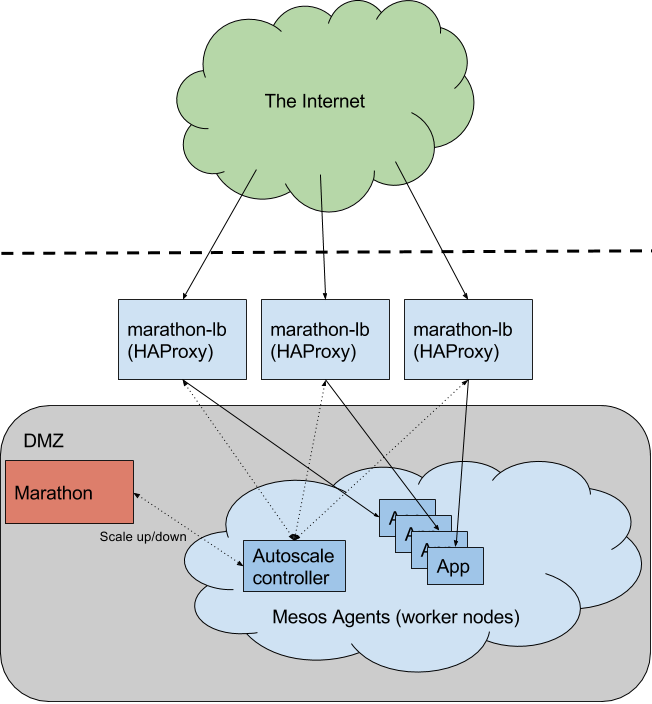
\includegraphics[keepaspectratio=true,scale=0.3]{img/marathon_lb_autoscale}
    \caption{Marathon LB Autoscale Architecture \cite{marathon_lb_autoscale}}
    \label{fig:marathon_lb_autoscale}
\end{figure}

\textbf{Microscaling in a Box} \cite {microscaling}\\
This service is one of many micro scaling implementations and provided by \textit{microscaling systems}.
It works by transferring the data between the applications via their own queue.
Then a target length can be defined which the tool tries to sustain then, which means it scales up or down a service based on the queue length.
The only metric supported is this queuing technique, which additionally takes advantage of the fact that launching further Docker container is relatively fast in comparison to launching an additional VM instance.
This is why the company claims to "automate scaling in real time" \cite{microscaling}.\\
The approach is suitable for services where the performance and workload mainly correlates with the incoming amount of data.
This is not the case in the whole SMACK stack, for example Spark could be overloaded with just a few messages in a computational bound application.
Further the usage of an additional queue between all services would slow down the stack and consume CPU and RAM resources.\\

None of the introduced tools or frameworks have a deeper look insight the SMACK stack to be able to tell whether or not a service is really under heavy load.
Those tools could be combined to get more insights but would therefore also consume a lot more resources, which is not desirable at all.
To be able to accurately monitor Akka for example, custom metrics have to be considered, which is very unlikely to be found in a generic autoscale tool.\\
The framework develped in the course of this thesis enables users to benefit from a deeper understanding of the components running in the SMACK stack to reliably detect when a service needs to be scaled.
This is done while being independent from TCP traffic based measurements or queue-length based approaches.
Further the framework is capable of handling user-defined metrics and is robust, as it can be hosted outside the cluster containing the SMACK stack.
